\chapter{Methodology}
\section{Motor Currents Reading}
\label{motor currents}

Before continue with more experiment and identification, there is one problem that needs to be solved first. The problem is that the arm only gives absolute value of the motor currents (\fref{fig:raw current}). In the figures, q1 refers to the first joint, q2 is the second joint and so on. Thus there is a need to identify the sign of the motor currents of each joints. Three methods were tried but only one was successful.

The first attempt was to give the motor current sign based on the sign of $\tau_{dyn}$ during non-contact condition. However, this poses a problem when the $\tau_{dyn}$ goes near zero as it will not be clear enough to identify the sign. The second method was to match the derivative of motor currents with derivative $\tau_{dyn}$ during pre-contact motion (e.g.: if $\tau_{dyn}$ is increasing, the motor currents has to be increasing too, and vice versa). Unfortunately, this principle working only if motor currents are very smooth and steady which is a very difficult condition.

After the first two attempts, it was found out that we can actually extract motor torques value from Denso and this time it includes the sign of it. The data is then plotted against motor currents with the sign of motor torques to see the relation. From \fref{fig:current vs torque} we can see that there is a good linearity between these two variables, and so we can now actually use motor torques instead of motor currents. By doing this, not only we do not need to take care of the currents sign problem anymore, we also simplify our problem since what we are interested in is the motor torques, not motor currents. However, since the value is not in the SI unit calibration is needed to adjust the value into the SI unit. 

\begin{figure}[H]
  \begin{subfigure}[t]{0.5\textwidth}
    \centering
    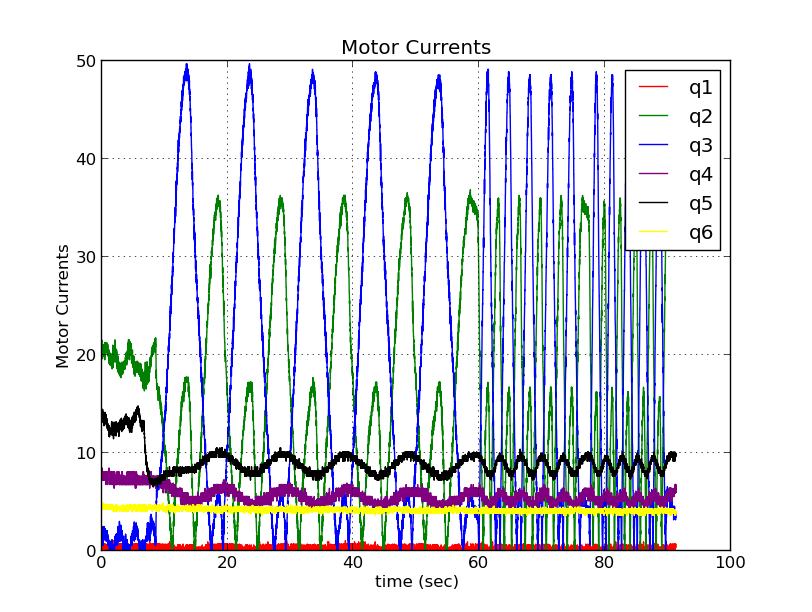
\includegraphics[width = \textwidth ]{raw_current} 
    \caption{Raw data of motor currents }
    \label{fig:raw current}
  \end{subfigure}
  \begin{subfigure}[t]{0.5\textwidth}
    \centering
    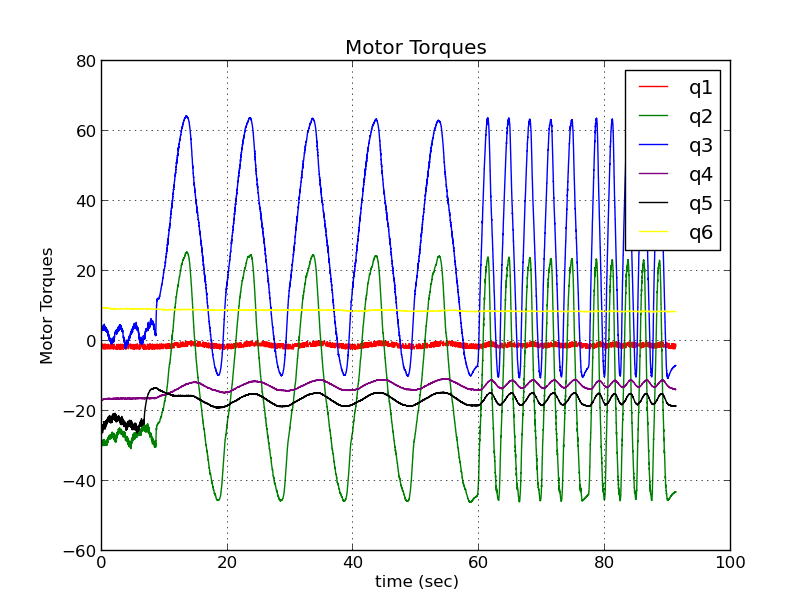
\includegraphics[width = \textwidth ]{raw_torque}
    \caption{Raw data of motor torques }
    \label{fig:raw torque}
  \end{subfigure}
  \caption{Reading of motor currents and torques}
\end{figure}

\begin{figure}[H]
    \centering
    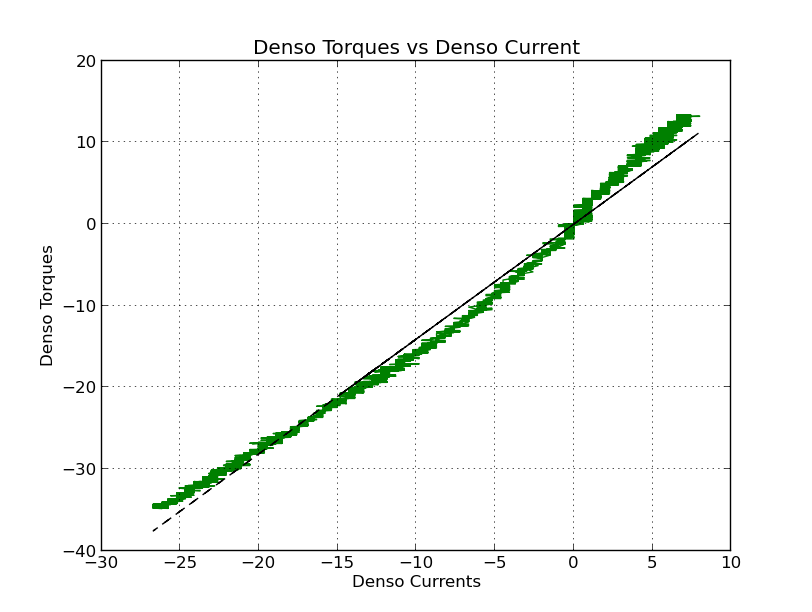
\includegraphics[width = 0.6\textwidth ]{current_torque}
    \caption{Motor torques vs motor currents with sign}
    \label{fig:current vs torque}
\end{figure}

\section{One-stage Experiment}
In the early process of the project, one-stage experiment was executed. The experiment can be described like this: The robot is moved into pre-contact position with any fixed object. The arm then moves slowly until contact is detected using F/T sensor. From there, a sinusoidal motion of the end-effector is performed to push the fixed object. This will make some joints to forcely push the robot. Figures below illustrate the simulation of the setup.

\begin{figure}[H]
  \begin{subfigure}[t]{0.5\textwidth}
    \centering
    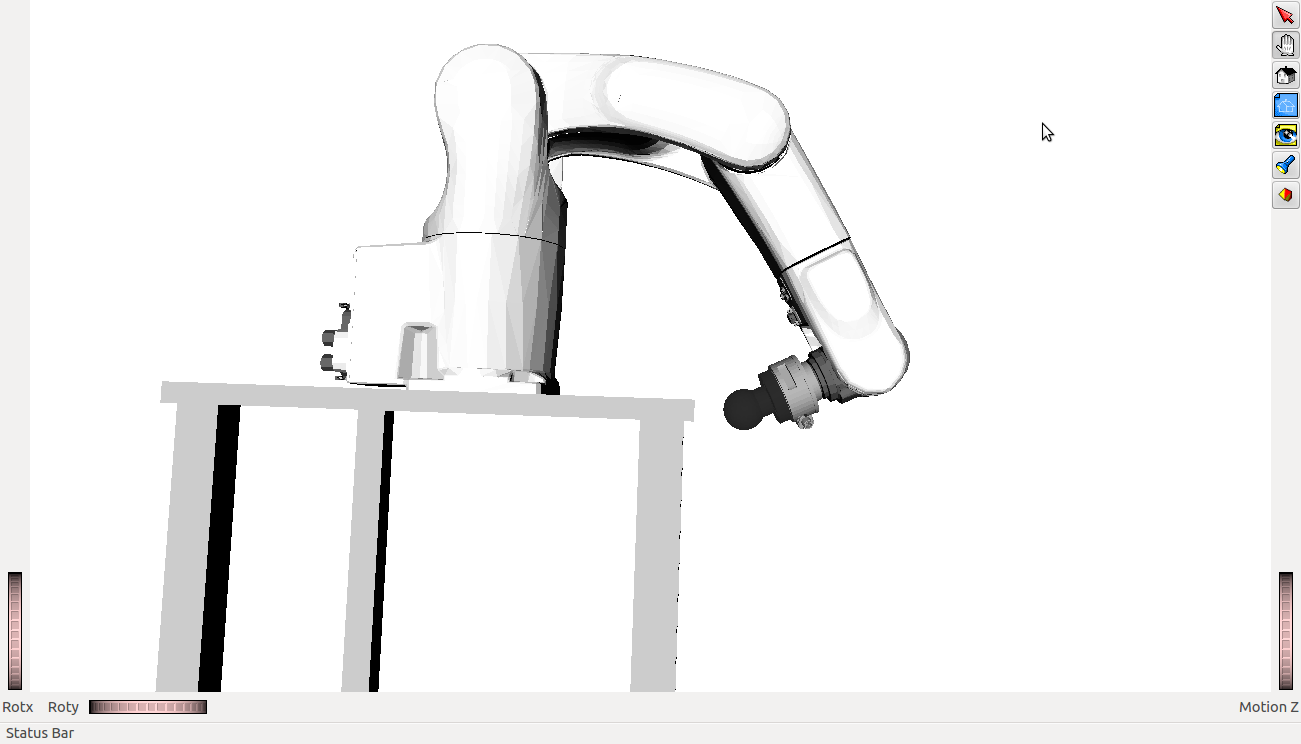
\includegraphics[width = \textwidth ]{one_stage_1} 
    \caption{Robot is in pre-contact position}
  \end{subfigure}
  \begin{subfigure}[t]{0.5\textwidth}
    \centering
    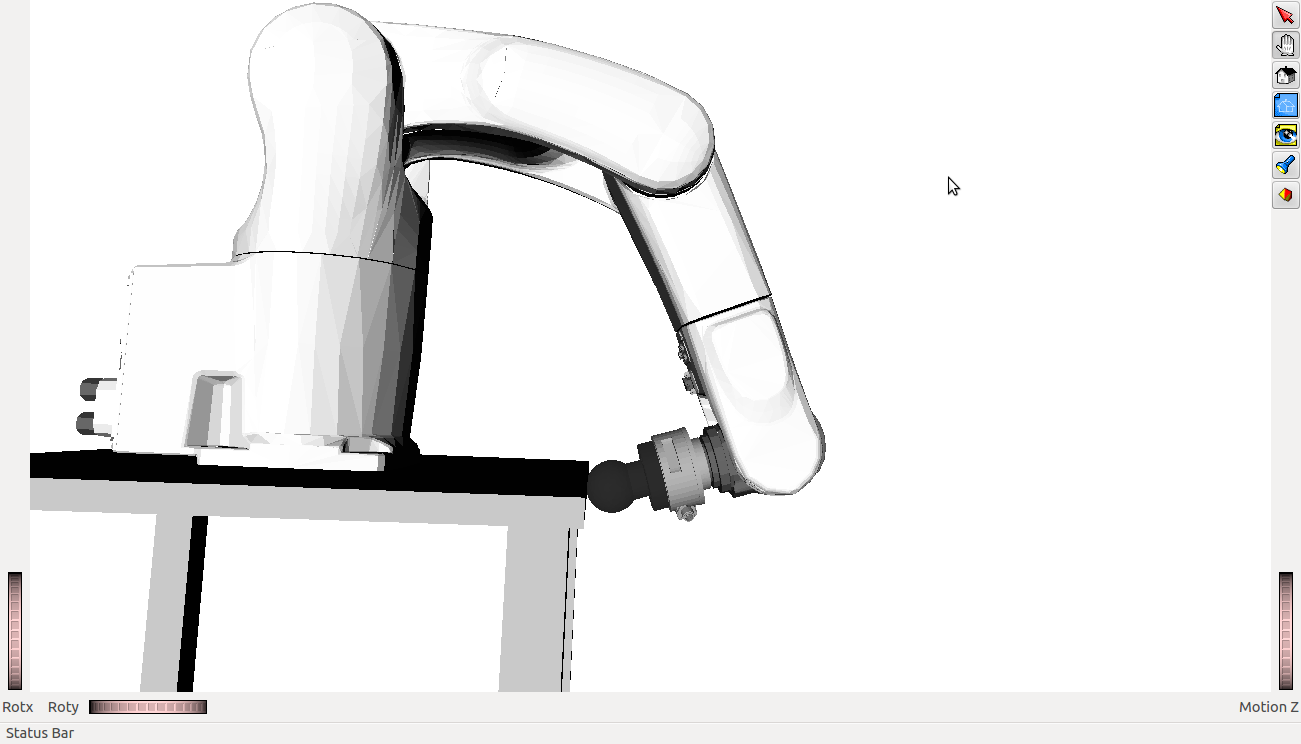
\includegraphics[width = \textwidth ]{one_stage_2}
    \caption{robot push the ground in a sinusoidal motion.}
  \end{subfigure}
  \caption{fig: One-stage experiment simulation}
\end{figure}

The purpose of this experiment is to capture all of the phenomenas (friction and contact force) in one experiment and so, identification of all parameters can be done for each joint in one experiment. Furthermore, depending on the setup one experiment can test for more than one joint at the same time, thus cutting the time to do the experiment. 

While it is feasible to do so, identification of the parameters turned out to be quite messy. The reasons are: 1) while all effects of the phenomena can be captured, it is difficult to distinguish one with each other, hence making it difficult in identifying each parameter and 2) performing the experiment for two or more joints at the same time was messy and not clean. Hence, the setup of experiment was then changed to be two-stage experiment.

\section{Two-Stage Experiment}
There are two stage of experiments which are required to identify the two important parameters : $K_{denso}$ and $\tau_{friction}$ (see chapter \ref{model}). The purpose of setting different type of experiment is to eliminate the effect of other parameter, thus the resulted data is affected only because of one parameter. That way the identification of each parameter tends to be easier and more accurate. The first stage of experiment is the high torque collection data to calibrate the motor torque ($K_{denso}$) while the second stage of experiment is the high velocity collection data which is performed to identify the $\tau_{friciton}$ characteristics. The data is captured in broad range of value to capture as many phenomena as possible.


\subsection{High Torque Collection Data}
\label{push exp}

The experiment is meant to collect the torque measurement from wide range to calibrate the motor torque. Firstly, the robot is moved to a position where the interested joint will receive a high torque from contact force. While the robot is fixed, the force is introduced at the end-effector of the arm such that the interested joint will experience a high torque. Motor torques are recorded from Denso arm and contact force/torque are recorded through ATI F/T sensor. The experiment is repeated in a different position for each joints. See figure below for illustration.

\begin{figure}[H]
    \centering
    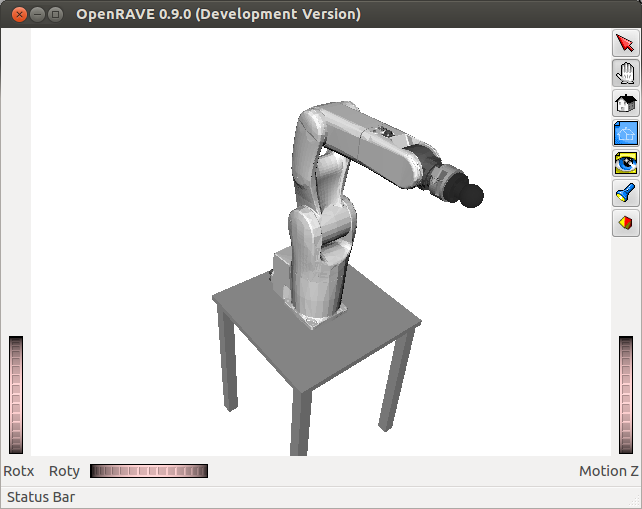
\includegraphics[width = 0.6\textwidth ]{high_torque}
    \caption{High torque collection data experiment for second joint}
\end{figure}


\subsection{High Velocity Collection Data}
\label{fric exp}

For this second experiment, the robot is moving in a free motion. Thus, a free rotation with different velocity is performed for each of respective joints. In this way, the effect of friction can be clearly caprtured. Motor torques, and joint positions which are crucial parameters are recorded from Denso manipulator for further analysis. See figure below for illustration.
\begin{figure}[H]
\centering  
  \begin{subfigure}[t]{0.3\textwidth}
    \centering
    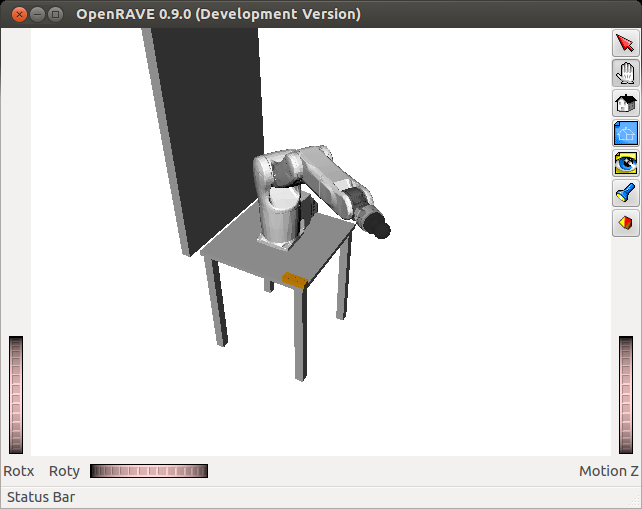
\includegraphics[width = \textwidth ]{high_vel_1} 
  \end{subfigure}
  \begin{subfigure}[t]{0.3\textwidth}
    \centering
    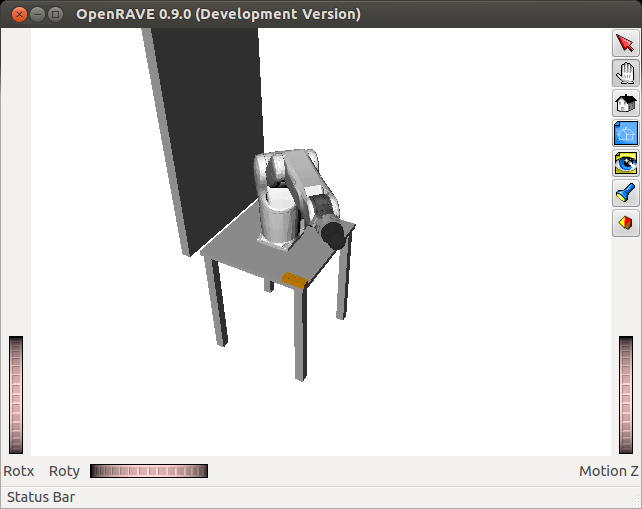
\includegraphics[width = \textwidth ]{high_vel_2}
  \end{subfigure}
  \begin{subfigure}[t]{0.3\textwidth}
    \centering
    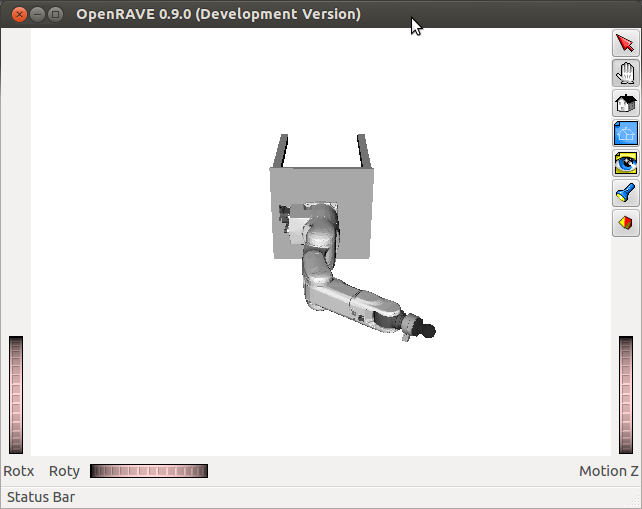
\includegraphics[width = \textwidth ]{high_vel_3}
  \end{subfigure}
  \caption{fig: High veloctiy collection data experiment for third joint}
\end{figure}


